% importa variabili globali
% definizione variabili globali
\def\GRUPPO {\textit{DazzleWorks}}

\def\PROGETTO {\textbf{Premi}}

\def\COMMITTENTE {Prof. Vardanega Tullio, \\ & Dr. Cardin Riccardo}

\def\EMAIL {dazzleworksgroup@gmail.com}

\def\LOGO {../../template/img/logo.png}

\def\INTESTAZIONE {../../template/img/intestazione.png}
\def\PIEDIPAGINA {../../template/img/piedipagina.png}

\def\G {{\small $_G$}}


% definizione variabili locali
\def\DOCUMENTO{Manuale Utente}
\def\VERSIONE{1.0.0}

\def\DESCRIZIONE{Documento che facilità l'utilizzo dell'applicazione da parte dell'utente.}

\def\REDATTORE {}
\def\VERIFICATORE {}
\def\RESPONSABILE {}

\def\USO {Esterno}

\def\DISTRIBUZIONE {\GRUPPO{}\\ & \COMMITTENTE{}\\}


% abilita (true) / disabilita (false) indice, lista tabelle, lista figure
\def\INDICE	{true}
\def\TABELLE {true}
\def\FIGURE {true}


% importa struttura
\documentclass[a4paper]{article}

% ----- definizioni -----
\def\TITLE		{\mbox{\GRUPPO}}
\def\SUBTITLE	{\SIGLA, \PROGETTO}


% ----- nuovi comandi -----
% fornisce il caption per riferirsi ad una particolare sezione
\newcommand{\numref}[1]{\textsf{\textsl{``\nameref{#1}'' (\ref{#1})}}}


% ----- package -----
\usepackage[T1]{fontenc}   % codifica dei font in uscita
\usepackage[utf8x]{inputenc}   % lettere accentate da tastiera
\usepackage[italian]{babel}   % lingua principale del documento
\usepackage[a4paper, top= 3cm, bottom= 3cm, left= 3cm, right= 3cm, bindingoffset= 5mm]{geometry} % impostazione margini

\usepackage{amssymb} %

\usepackage{booktabs} % comandi aggiuntivi per le tabelle

\usepackage{calc} % espressioni aritmetiche
\usepackage{caption} % descrizione figure, ecc
\usepackage{chapterbib} % inclusione delle bibliografie

\usepackage{datatool} % manipolazione dati
\usepackage{dcolumn} % array in tabular

\usepackage{epstopdf} % conversione eps--> pdf
\usepackage{enumitem} % personalizzazione liste
\usepackage{eurosym} % simbolo euro

\usepackage{fancyhdr}   %personalizzazione dello stile
\usepackage{float} % definizione di oggetti floating (es. figure, tabelle)
\usepackage[bottom]{footmisc} % personalizzazione note

\usepackage[toc]{glossaries}	% glossario
\usepackage{graphicx, subfigure} % pacchetto grafica testo
\usepackage{grffile} % estende gestione filename graphic

\usepackage[colorlinks=true, urlcolor=blue, citecolor=black, linkcolor=black, hyperindex, breaklinks]{hyperref} % gestione dei link

\usepackage{ifthen}	% costrutto ifthenelse

% \usepackage{listings} % inserimento pezzi di codice
\usepackage{longtable} % tabelle su più pagine

\usepackage{pgf} % grafica postscript e PDF
\usepackage{pgfplots}	% composizione di grafici
\pgfplotsset{/pgf/number format/use comma, compat=newest}	% opzioni per i grafici

\usepackage{multirow} % span multiriga

\usepackage{tabularx, array} % crea paragrafi a colonne
\usepackage{titlesec} % personalizzazione titoli
\usepackage{tikz} % gestione delle formule
\usepackage{totpages} % conta numero pagine

\usepackage{soul} % gestione letterspacing
\usepackage{subfigure} % gestione delle sottofigure

\usepackage{verbatim} % inserimento testo verbatim, non interpretato

\usepackage{wallpaper} % gestione background

\usepackage{xspace} % spazi automatici per le macro


% ----- posizione etichette -----
\captionsetup{tableposition=top, figureposition=bottom, font=small}


% ----- glossario -----
\loadglsentries{../../glossario/glossario.tex}
\renewcommand*{\glssymbolsgroupname}{Simboli}


% ----- stile pagina -----
\pagestyle{fancy}

	% header
	\fancypagestyle {firststyle} {	% definizione stile "firststyle"
		\fancyhf{}
	}

	% indentazione paragrafo
	%\setlength{\parindent} {0pt}
	\setlength{\headheight} {25pt}

	% intestazione
	\lhead{}
	\rhead{\nouppercase{\leftmark}}
	\renewcommand{\headrulewidth}{0pt}  % no linea sotto intestazione

	% piè di pagina
	\lfoot{\footnotesize{{\DOCUMENTO} \\ {\VERSIONE}}}
	\cfoot{}
	\rfoot{\thepage}
	\renewcommand{\footrulewidth}{0pt}   % no linea sopra piè di pagina


% ----- inizio documento -----
% ----- prima pagina -----
\begin{document}
\thispagestyle{firststyle}

\begin{center}

%   \vspace{7cm}
	\textbf{{\fontsize{40pt}{41pt}\selectfont \PROGETTO}} \\
	\rule{8cm}{3pt}
   
   \vspace{4cm}
   \includegraphics[height= 4cm] {\LOGO}
   
	\vspace{1cm}
   {\fontsize{30pt}{31pt}\selectfont \textbf{\GRUPPO}}
	
	\vspace{5cm}
	{\fontsize{18pt}{24pt}\selectfont \textbf{\DOCUMENTO}}
	
%	\vspace{1cm}
	\begin{center}
		\begin{tabular}{r|l}
				\textbf{Versione} & \VERSIONE \\
				\textbf{Redattori} & \REDATTORE \\
				\textbf{Verificatori} & \VERIFICATORE \\
				\textbf{Responsabili} & \RESPONSABILE \\
				\textbf{Uso} & \USO \\
				\textbf{Lista di distribuzione} & \DISTRIBUZIONE
		\end{tabular}
	\end{center}

	\vspace{1cm}
	\textbf{\DESCRIZIONE}

\end{center}


\newpage

% ----- pagine successive -----
\ULCornerWallPaper{1}{\INTESTAZIONE}
\LLCornerWallPaper{1}{\PIEDIPAGINA}

%\thispagestyle{empty}

\newpage

% diario delle modifiche


% numerazione pagine indici
\pagenumbering{Roman}



% importa indici
% definizione indice
\ifthenelse{\equal{\INDICE}{true}}
	{\tableofcontents \newpage}{}

% definizione lista tabelle
%\ifthenelse{\equal{\TABELLE}{true}} 
%	{\listoftables \newpage}{}

% definizione lista figure
\ifthenelse{\equal{\FIGURE}{true}}
	{\listoffigures \newpage}{}


% numerazione pagine
\pagenumbering{arabic}

	% formato visualizzazione
	\rfoot{\thepage ~di~\pageref{TotPages}}


% separatore
\iffalse
	AOjvdYTJD7mcIIYItfsNiYPbmTTogRSP9hrrb2XPE1laMyQ9NHrPgTCTxnW0eV1YcM3Wqh7t5qThjczeXWq3O5FJ7BBQjoWZovC5
\fi

\section{Introduzione}
\subsection{Scopo del documento}
	Il documento ha lo scopo di definire l'architettura generale e i \gls{design pattern} da utilizzare secondo i quali verrà sviluppato il software del progetto Premi.

\subsection{Scopo del prodotto}
Lo scopo del progetto è realizzare un software per un sistema di rappresentazione di \gls{slide} sfruttando la tecnologia  \gls{HTML5}. Lo scopo principale è quello di creare un prodotto che sia di qualità comparabile, in prestazioni, funzionalità ed effetti visivi, ai maggiori concorrenti già presenti sul mercato (Prezi, Powerpoint, Keynote, Impress, ...).

\subsection{Glossario}
Per prevenire ed evitare qualsiasi dubbio e per permettere una maggiore chiarezza e comprensione del testo su termini ambigui, abbreviazioni e acronimi utilizzati nei vari documenti, essi sono stati raccolti nel \textit{Glossario v2.0.0} nel quale si possono trovare tutte le informazioni desiderate.
Al fine di rendere subito evidente un termine presente nel \textit{Glossario}, esso verrà marcato con il pedice \G\footnote{Per le istruzioni si rimanda al documento \textit{Norme di Progetto v2.0.0} .}.

\subsection{Riferimenti}

\subsubsection{Normativi}
	\begin{itemize}
		\item \textbf{Analisi dei Requisiti:} \textit{Analisi dei Requisiti v3.0.0};
		\item \textbf{Norme di Progetto:} \textit{Norme di Progetto v2.0.0}.
	\end{itemize}

\subsubsection{Informativi}
	\begin{itemize}
		\item \textbf{Design Patterns, elementi per il riuso di software ad oggetti:} Gamma, Helm, Johnson, Vlissides;
		\item \textbf{SWEBOK v3, Guide to the Software Engineering Body of Knowledge:} IEEE Computer Society;
		\item \textbf{Ingegneria del software} Ian Sommerville, Parte terza: \textit{progettazione};
		\item \textbf{Slide del corso:}
				\begin{itemize}
					\item \textbf{Diagrammi delle classi}: \url{http://www.math.unipd.it/~tullio/IS-1/2014/Dispense/E2a.pdf};
					\item \textbf{Diagrammi dei package}: \url{http://www.math.unipd.it/ ~tullio/IS-1/2014/Dispense/E2b.pdf};
					\item \textbf{Pattern}:
					\begin{itemize}
						\item \textit{Architetturali}
							\begin{itemize}
								\item \url{http://www.math.unipd.it/~tullio/IS-1/2014/Dispense/E9.pdf};
								\item \url{http://www.math.unipd.it/~rcardin/pdf/Design\%20Pattern\%20Architetturali\%20-\%20Model\%20View\%20Controller\_4x4.pdf};
							\end{itemize}
						\item \textit{Strutturali}:
						\begin{itemize}
						\item \url{http://www.math.unipd.it/~tullio/IS-1/2014/Dispense/E6.pdf};
						\end{itemize}
						\item \textit{Creazionali}:
						\begin{itemize}
						\item \url{http://www.math.unipd.it/~tullio/IS-1/2014/Dispense/E7.pdf};
						\end{itemize}
						\item \textit{Comportamentali}:
						\begin{itemize}
						\item \url{http://www.math.unipd.it/~tullio/IS-1/2014/Dispense/E8.pdf};
						\end{itemize}
					\end{itemize}
					\item \textbf{Documentazione di Chart.js}: \url{http://chartjs.org/docs};
					\item \textbf{Documentazione di Angular.js}: \url{https://docs.angularjs.org/guide};
					\item \textbf{Documentazione di Reveal.js}: \url{http://github.com/hakimel/reveal.js};
					\item \textbf{Documentazione di Fabric.js}: \url{http://fabricjs.com};
					\item \textbf{Manuale di MongoDb}: \url{https://docs.mongodb.org/manual};
					\item \textbf{Documentazione di Foundation}: \url{http://foundation.zurb.com/docs};
					\item \textbf{Documentazione di Php}: \url{http://php.net/docs.php}.
				\end{itemize}

	\end{itemize}

\newpage
\section{Start}
Di seguito viene spiegato l'utilizzo delle principali funzioni dell'applicazione
\section{Registrazione}
Per creare un nuovo account selezionare il tasto \textbf{Sign Up} posizionato in alto a destra dello schermo.

\noindent Ora bisogna compilare un piccolo form che richiede alcuni dati necessari per poter effettuare la registrazione: username, email, first name, last name, password e verifica password.

\noindent Una volta compilati tutti i campi richiesti premere il bottone \textbf{Sign Up} situato sotto il form.

\section{Autenticazione}
Se si possiede già un account è possibile effettuare l'autenticazione.

\noindent Per autenticarsi premere il pulsante \textbf{Login} situato in alto a destra dello schermo accanto al pulsante di registrazione.

\noindent Ora sono richiesti i dati d'accesso.

\begin{figure}[h] 
	\centering 
	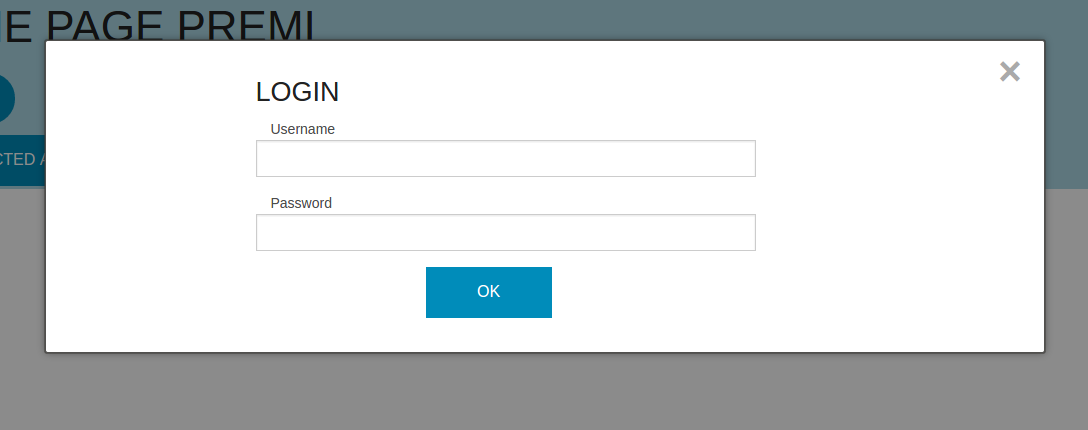
\includegraphics[scale=0.40] {img/MULogin.png}
	\caption{UC1 - Registrazione} 
\end{figure}

\noindent Una volta inseriti premere il pulsante \textbf{Login} situato sotto il form.

\section{Creazione di un Progetto}

Effettuata l'autenticazione è possibile cominciare a creare progetti.


\noindent Per creare un progetto selezionare dal menù in alto \textbf{New Project} e inserite un titolo per il progetto.


\section{Creazione di una Presentazione}

Una volta creato un progetto verrà automaticamente aperto l'editor che permette di creare le slide della presentazione.

\section{Creazione di un'Infografica}

Per creare un'infografica è sufficiente aprire un progetto e premere il pulsante \textbf{New Infographic}; dal menù laterale e verrà aperto l'editor con cui è possibile modificare l'infografica.

\section{Ricerca di un progetto}

È possibile fare una ricerca tra i progetti salvati da altri utenti.

\noindent Per fare ciò è sufficiente compilare il filtro di ricerca, presente sulla propria home page, e premere il pulsante \textbf{Search}.

Verrà visualizzata una lista di progetti che rispettano i parametri inseriti.

\noindent A questo punto basta selezionarne uno e scegliere la modalità di visualizzazione.
\newpage
\section{Editor Presentazioni}
Di seguito vengono spiegati l'utilizzo degli strumenti di modifica delle presentazioni.

\subsection{Layout principale}
Una volta avviato l'editor delle presentazioni la pagina che appare si presenta semplice ed intuitiva. A sinistra si trova un menù verticale con tutti i pulsanti che permettono di modificare la slide corrente. Al centro dello schermo invece si trova lo spazio di gestione dei contenuti della slide, dove è possibile interagire con i contenuti.

\begin{figure}[H] 
	\centering 
	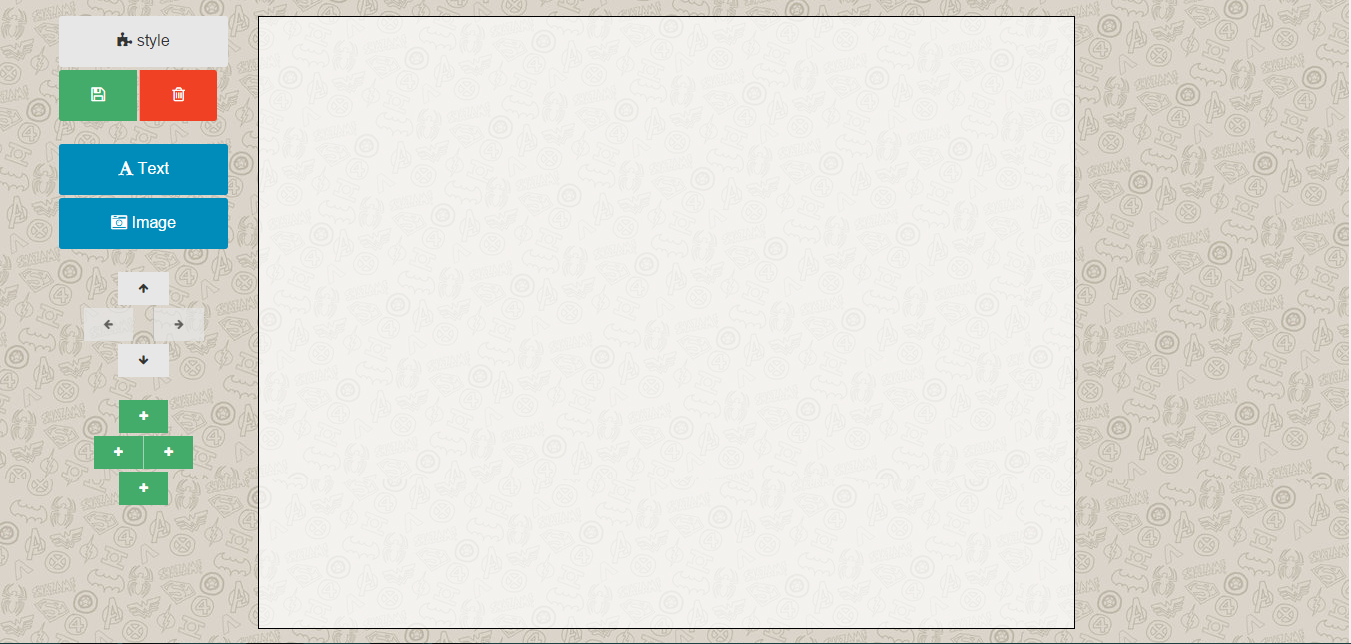
\includegraphics[scale=0.40] {img/layout_editor.png}
	\caption{Layout principale} 
\end{figure}

Di seguito verrà analizzato, dall'alto verso il basso, ciascun pulsante presente.

\subsection{Menù laterale}
\begin{itemize}
 \item \textbf{Style}\\
    Il pulsante \textbf{Style} permette di scegliere gli effetti di transizione e il tema da applicare alla slide. Una volta scelte le modifiche si deve confermare con il tasto \textbf{OK}.	
    \begin{figure}[H] 
    	\centering 
    	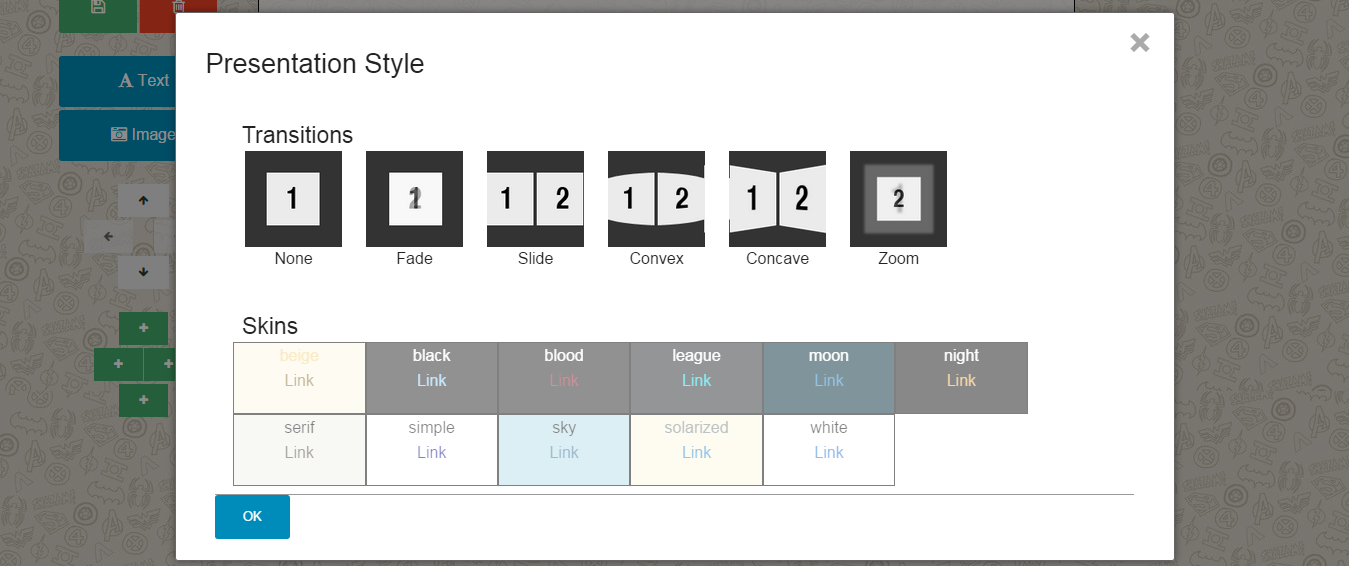
\includegraphics[scale=0.40] {img/editor_style.png}
    	\caption{Menù laterale - Style} 
    \end{figure}
	
 \item \textbf{Salva}\\
	Il pulsante di colore verde è il pulsante che permette di salvare le modifiche apportate alla slide. 	
	\begin{figure}[H] 
		\centering 
		
\includegraphics[scale=0.40] {img/editor_save.png}
		\caption{Menù laterale - Salva} 
	\end{figure}
	
	 \item \textbf{Elimina}\\
	 Il pulsante di colore rosso è il pulsante che permette di eliminare tutto il contenuto della slide corrente.  	
	 \begin{figure}[H] 
	 	\centering 
	 	
\includegraphics[scale=0.40] {img/editor_del.png}
	 	\caption{Menù laterale - Elimina} 
	 \end{figure}
	
 \item \textbf{Text}\\
    Il pulsante \textbf{Text} permette di inserire del testo nella slide. Una volta inserito il testo nell'apposita casella si deve confermare con il tasto \textbf{OK}.
    \begin{figure}[H] 
	\centering 
	
\includegraphics[scale=0.40] {img/editor_text.png}
	\caption{Menù laterale - Text} 
    \end{figure}
    
    
 \item \textbf{Image}\\
    Il pulsante \textbf{Image} permette di aggiungere un'immagine alla \gls{slide} corrente tra quelle già caricate o di caricarne un'altra presente sul file system dell'utente. Una volta scelta l'immagine questa verrà inserita automaticamente nella slide.
   \begin{figure}[H] 
	\centering 
	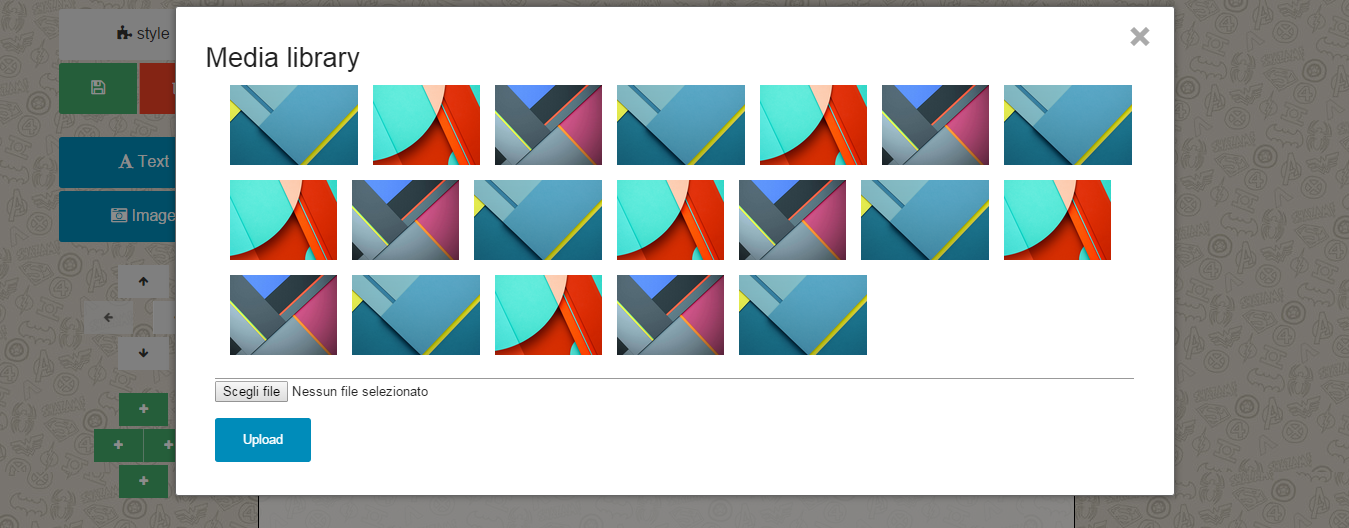
\includegraphics[scale=0.40] {img/editor_img.png}
	\caption{Menù laterale - Image} 
    \end{figure}
    
\newpage

  \item \textbf{Navigazione delle slide}\\
  I pulsanti freccia permettono di navigare tra le slide già create della presentazione. Ad ogni tasto corrisponde una direzione di spostamento.
  \begin{figure}[h] 
  	\centering 
  	
\includegraphics[scale=0.80] {img/editor_move.png}
  	\caption{Menù laterale - Aggiunta di una slide} 
  \end{figure}
 
 
 
\item \textbf{Aggiunta di una slide}\\
 Il pulsante con il simbolo \textbf{+} permette di aggiungere una nuova slide nella direzione corrispondente al pulsante premuto.
 \begin{figure}[h] 
 	\centering 
 	
\includegraphics[scale=0.80] {img/editor_add.png}
 	\caption{Menù laterale - Aggiunta di una slide} 
 \end{figure}

\end{itemize}


\newpage

\subsection{Modifica di un componente}
Per modificare un componente è sufficiente selezionarlo nella \gls{slide} e modificarne gli attributi dal menù che comparirà sulla destra.

\subsubsection{Text}
La grandezza, la posizione e la rotazione della casella di testo possono essere modificate con il mouse tramite gli appositi punti di ancoraggio che compaiono una volta selezionato il testo. Il trascinamento in un angolo provoca una variazione della dimensione proporzionale tra larghezza ed altezza.

\begin{figure}[H] 
	\centering 
	
\includegraphics[scale=0.80] {img/text_anchor.png}
	\caption{Modifica di un componente - Modifica testo con mouse} 
\end{figure}

\noindent In alternativa si possono modificare le proprietà del testo dal menù laterale di destra, nel dettaglio:
		
		\begin{itemize}
			\item \textbf{ScaleX}: modifica la larghezza della casella di testo;
			\item \textbf{ScaleY}: modifica l'altezza della casella di testo;
			\item \textbf{Freccia verso l'alto}: sposta la casella di testo di un livello verso l'alto;
			\item \textbf{Freccia verso il basso}: sposta la casella di testo di un livello verso il basso;
			\item \textbf{Delete}: elimina la casella di testo;
			\item \textbf{Text}: modifica il testo contenuto nella casella di testo;
			\item \textbf{Tasto B}: modifica lo stile del testo in BOLD;
			\item \textbf{Tasto I}: modifica lo stile del testo in ITALIC;
			\item \textbf{Tasto U}: modifica lo stile del testo in UNDERLINE;
			\item \textbf{Size}: modifica la grandezza del testo;
			\item \textbf{Select Font}: modifica il font del testo.
		\end{itemize}
		 \begin{figure}[h] 
		    \centering 
		    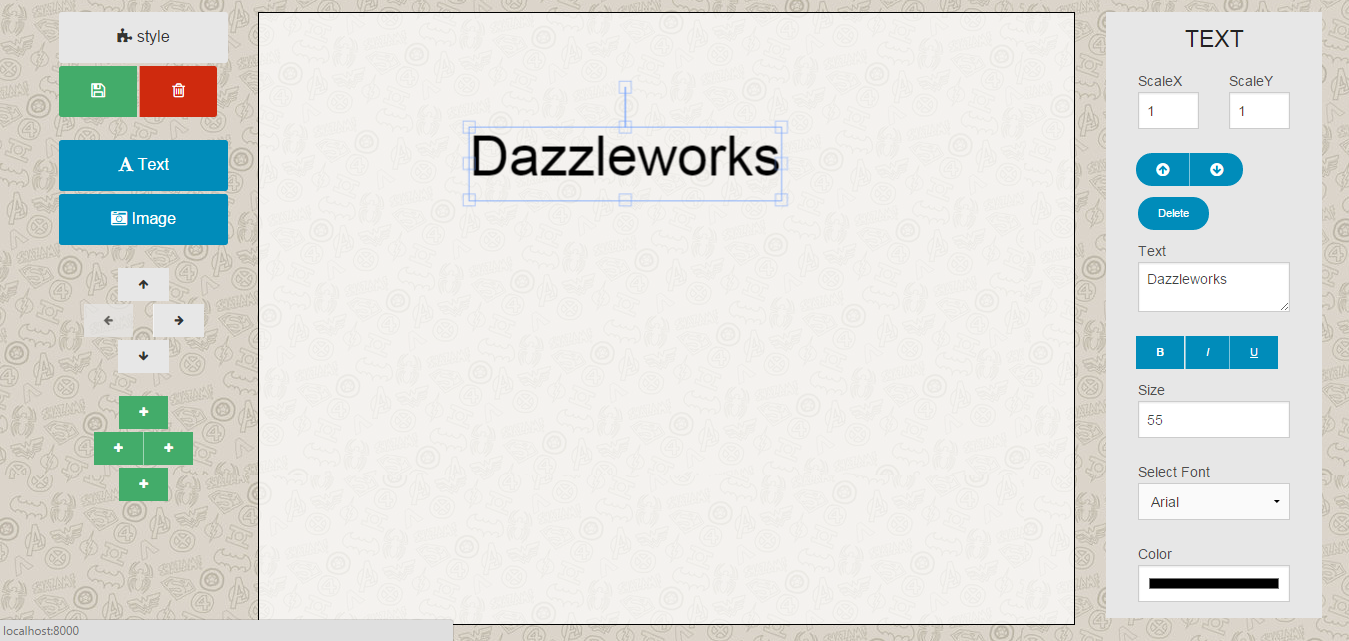
\includegraphics[scale=0.40] {img/text_edit.png}
		    \caption{\gls{Slide} Editor - Modifica testo da menù} 
		\end{figure}
		
		
\newpage 

\subsubsection{Image}
La grandezza, la posizione e la rotazione dell'immagine possono essere modificate con il mouse tramite gli appositi punti di ancoraggio che compaiono una volta selezionata l'immagine. Il trascinamento in un angolo provoca una variazione della dimensione proporzionale tra larghezza ed altezza.

\begin{figure}[H] 
	\centering 
	
\includegraphics[scale=0.80] {img/img_anchor.png}
	\caption{Modifica di un componente - Modifica immagine con mouse} 
\end{figure}

\noindent In alternativa si possono modificare le proprietà dell'immagine dal menù laterale di destra, nel dettaglio:

		\begin{itemize}
			\item \textbf{ScaleX}: modifica la larghezza dell'immagine;
			\item \textbf{ScaleY}: modifica l'altezza dell'immagine;
			\item \textbf{Freccia verso l'alto}: sposta l'immagine di un livello verso l'alto;
			\item \textbf{Freccia verso il basso}: sposta l'immagine di un livello verso il basso;
			\item \textbf{Delete}: elimina l'immagine;
		\end{itemize}
		
\begin{figure}[H] 
	\centering 
	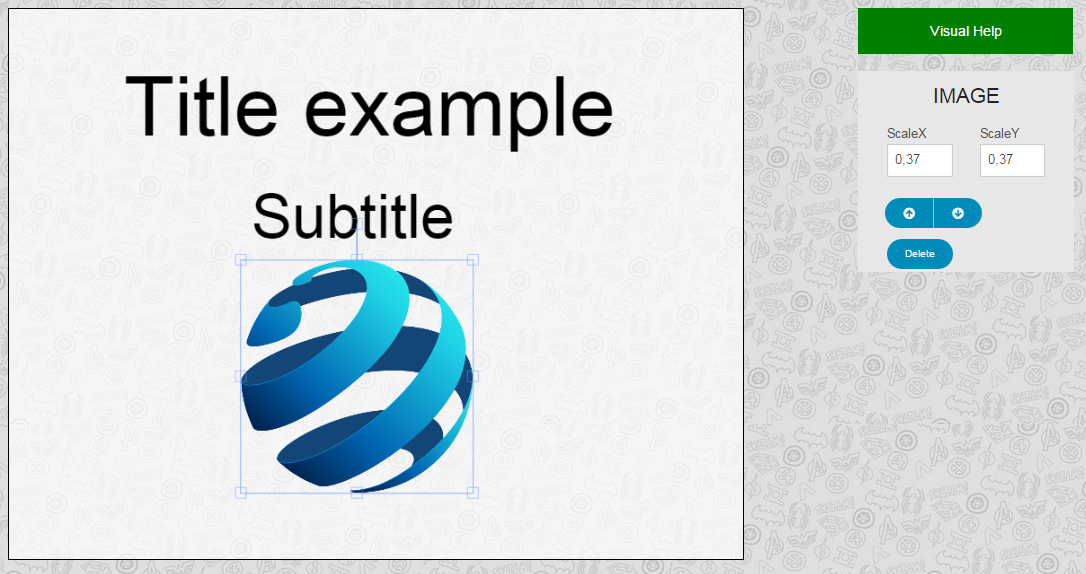
\includegraphics[scale=0.40] {img/img_edit.png}
	\caption{\gls{Slide} Editor - Modifica immagine da menù} 
\end{figure}	



\newpage
\section{Editor Infografiche}
\noindent
Di seguito vengono spiegati l'utilizzo degli strumenti di modifica delle infografiche.

\subsection{Menù laterale}
  \begin{itemize}
      \item \textbf{Slide}\\
	  Premendo il pulsante del menù laterale \textbf{Slide} verrà visualizzata una finestra nella quale si potrà scegliere da quali slide della presentazione ricavare le informazioni più rilevanti che verranno poi inserite nell'infografica secondo il template scelto.
      \item \textbf{Settings}\\
	  Premendo il pulsante del menù laterale \textbf{Settings} verrà visualizzata una finestra nella quale si possono modificare alcune opzioni riguardante l'infografica, tra le quali, dimensione della carta e template.
      \item \textbf{Save}\\
	  Premendo il pulsante del menù laterale \textbf{Save} verrà salvata l'infografica all'interno del progetto generando un file PNG ed un PDF a patire dalla superficie interattiva.
      \item \textbf{Print}\\
	  Premendo il pulsante del menù laterale \textbf{Print} verrà aperta la finestra di stampa del browser per stampare l'infografica.
      \item \textbf{Modifica di un componente}\\
	  Per modificare un componente (slide) è sufficiente trascinare una slide da quelle disponibili nel progetto corrente nella superfice interattiva.
  \end{itemize}
\newpage
\section{Gestione dell'Account}
\input{sections/Account.tex}

%\newpage

% ...

%\printglossaries

\end{document}